\documentclass{article}
%\documentclass{article}
\usepackage{amsmath, amsthm, amssymb}
\usepackage{tikz}
\usepackage{subfig}
\usepackage{verbatim}
\usepackage[all]{xy}
\usetikzlibrary{positioning}

\newcommand{\set}[1] {{\left\{#1\right\}}}


\begin{document}


\title{Tiling Problems: Data Intensive Computing on Analytic Graphs}
\author{Max Hutchinson}
\date{\today}
\maketitle

\section*{Background}

Tiling problems are combinatorial problems of the form: Given a 2-dimensional region and a set of tiles, how many configurations (tilings) of tiles cover the region without overlapping.  For example, there are eight tilings of a unit regular octagon with square and rhombic tiles, as shown in Figure~\ref{fig:examp}.
\begin{figure}[h!]
\begin{center}
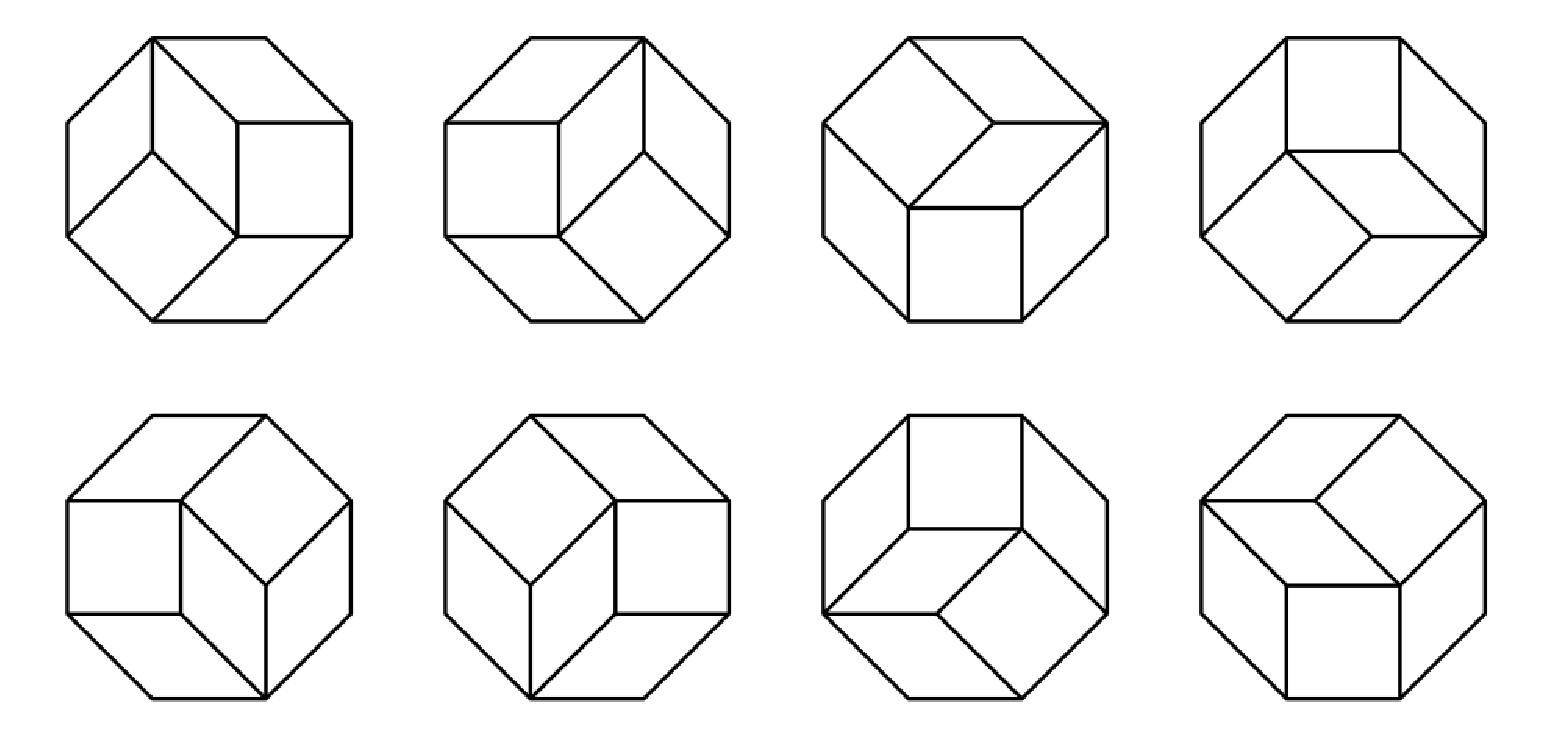
\includegraphics[width=0.7\textwidth]{unit_tilings}
\end{center}
\caption{The eight tilings of the unit octagon by squares and $45^\circ$ rhombi.}
\label{fig:examp}
\end{figure} 
Tiling problems are popular models of quasicrystals~\cite{Shechtman1984,Levine1984}, a relatively recently discovered solid phase for which Dan Shechtman won the Nobel Prize in Chemistry in 2011.

The number of tilings of a region grows exponentially with the area: for a similar octagon of edge length 2 there are 5383 tilings; edge length 3 has 273976272 tilings~\cite{Dest04}.  Needless to say, the tilings can not be counted explicitly.  Fortunately, there is a correspondence to a class of problems known as `partition problems,' and a graph-based algorithm for solving them~\cite{Dest01}.

To solve octagonal tiling problems, one constructs a digraph of binary swaps.  Examples of such graphs are shown in Figures~\ref{fig:graph} and ~\ref{fig:sgrhs}.
\begin{figure}[h!]
\begin{center}
$$\xymatrix{
& \ar@/_/[dl] \left(0, 0, 1, 1, 2, 2\right) \ar@/^/[dr]& \\
\left(0, 1, 0, 1, 2, 2\right) \ar[d] \ar@/_/[dr] & &  \ar@/^/[dl] \ar[d] \left(0, 0, 1, 2, 1, 2\right) \\
\left(1, 0, 0, 1, 2, 2\right) & \left(0, 1, 0, 2, 1, 2\right) &  \left(0, 0, 2, 1, 1, 2\right)}$$ 
\end{center}
\caption{First 3 layers of a graph of size $(2,2,2)$.}
\label{fig:graph}
\end{figure}

\begin{figure}
  \centering
    \subfloat[(1,1,1)]{\label{fig:sgrph-1,1,1}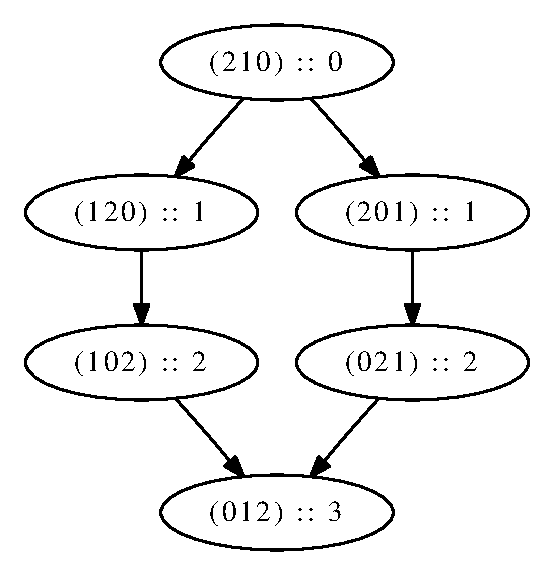
\includegraphics[width=0.30\textwidth]{sort-1,1,1.eps}}
    \subfloat[(1,2,1)]{\label{fig:sgrph-1,2,1}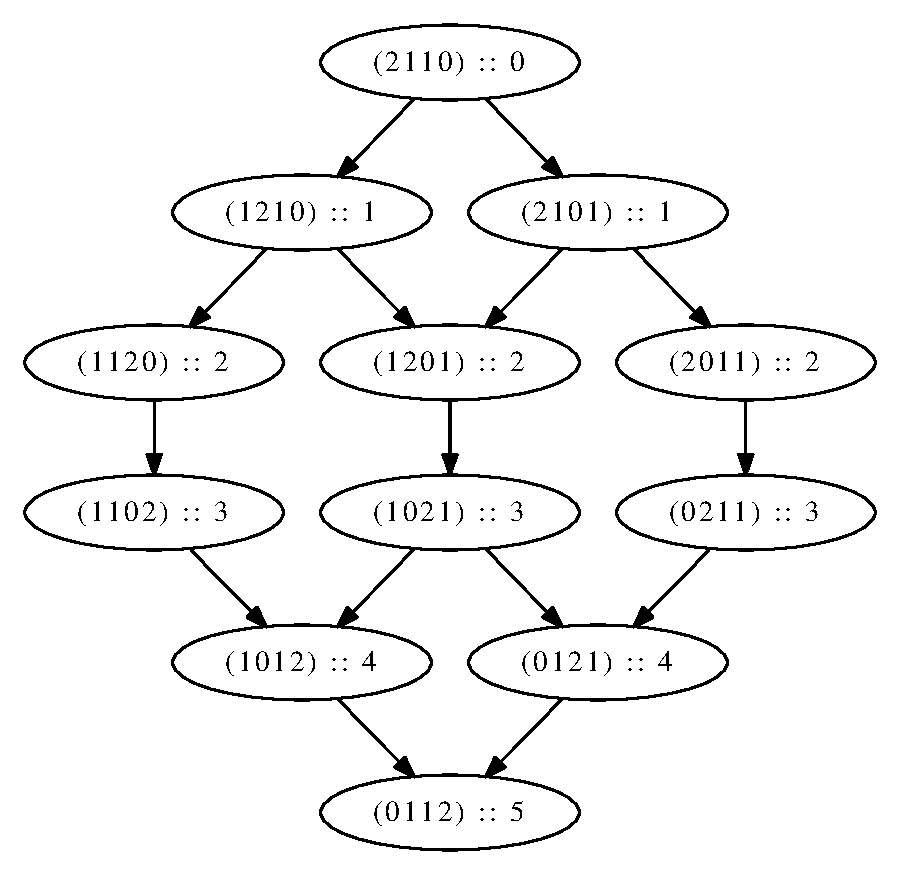
\includegraphics[width=0.30\textwidth]{sort-1,2,1.eps}}
    \subfloat[(2,2,2)]{\label{fig:sgrph-2,2,2}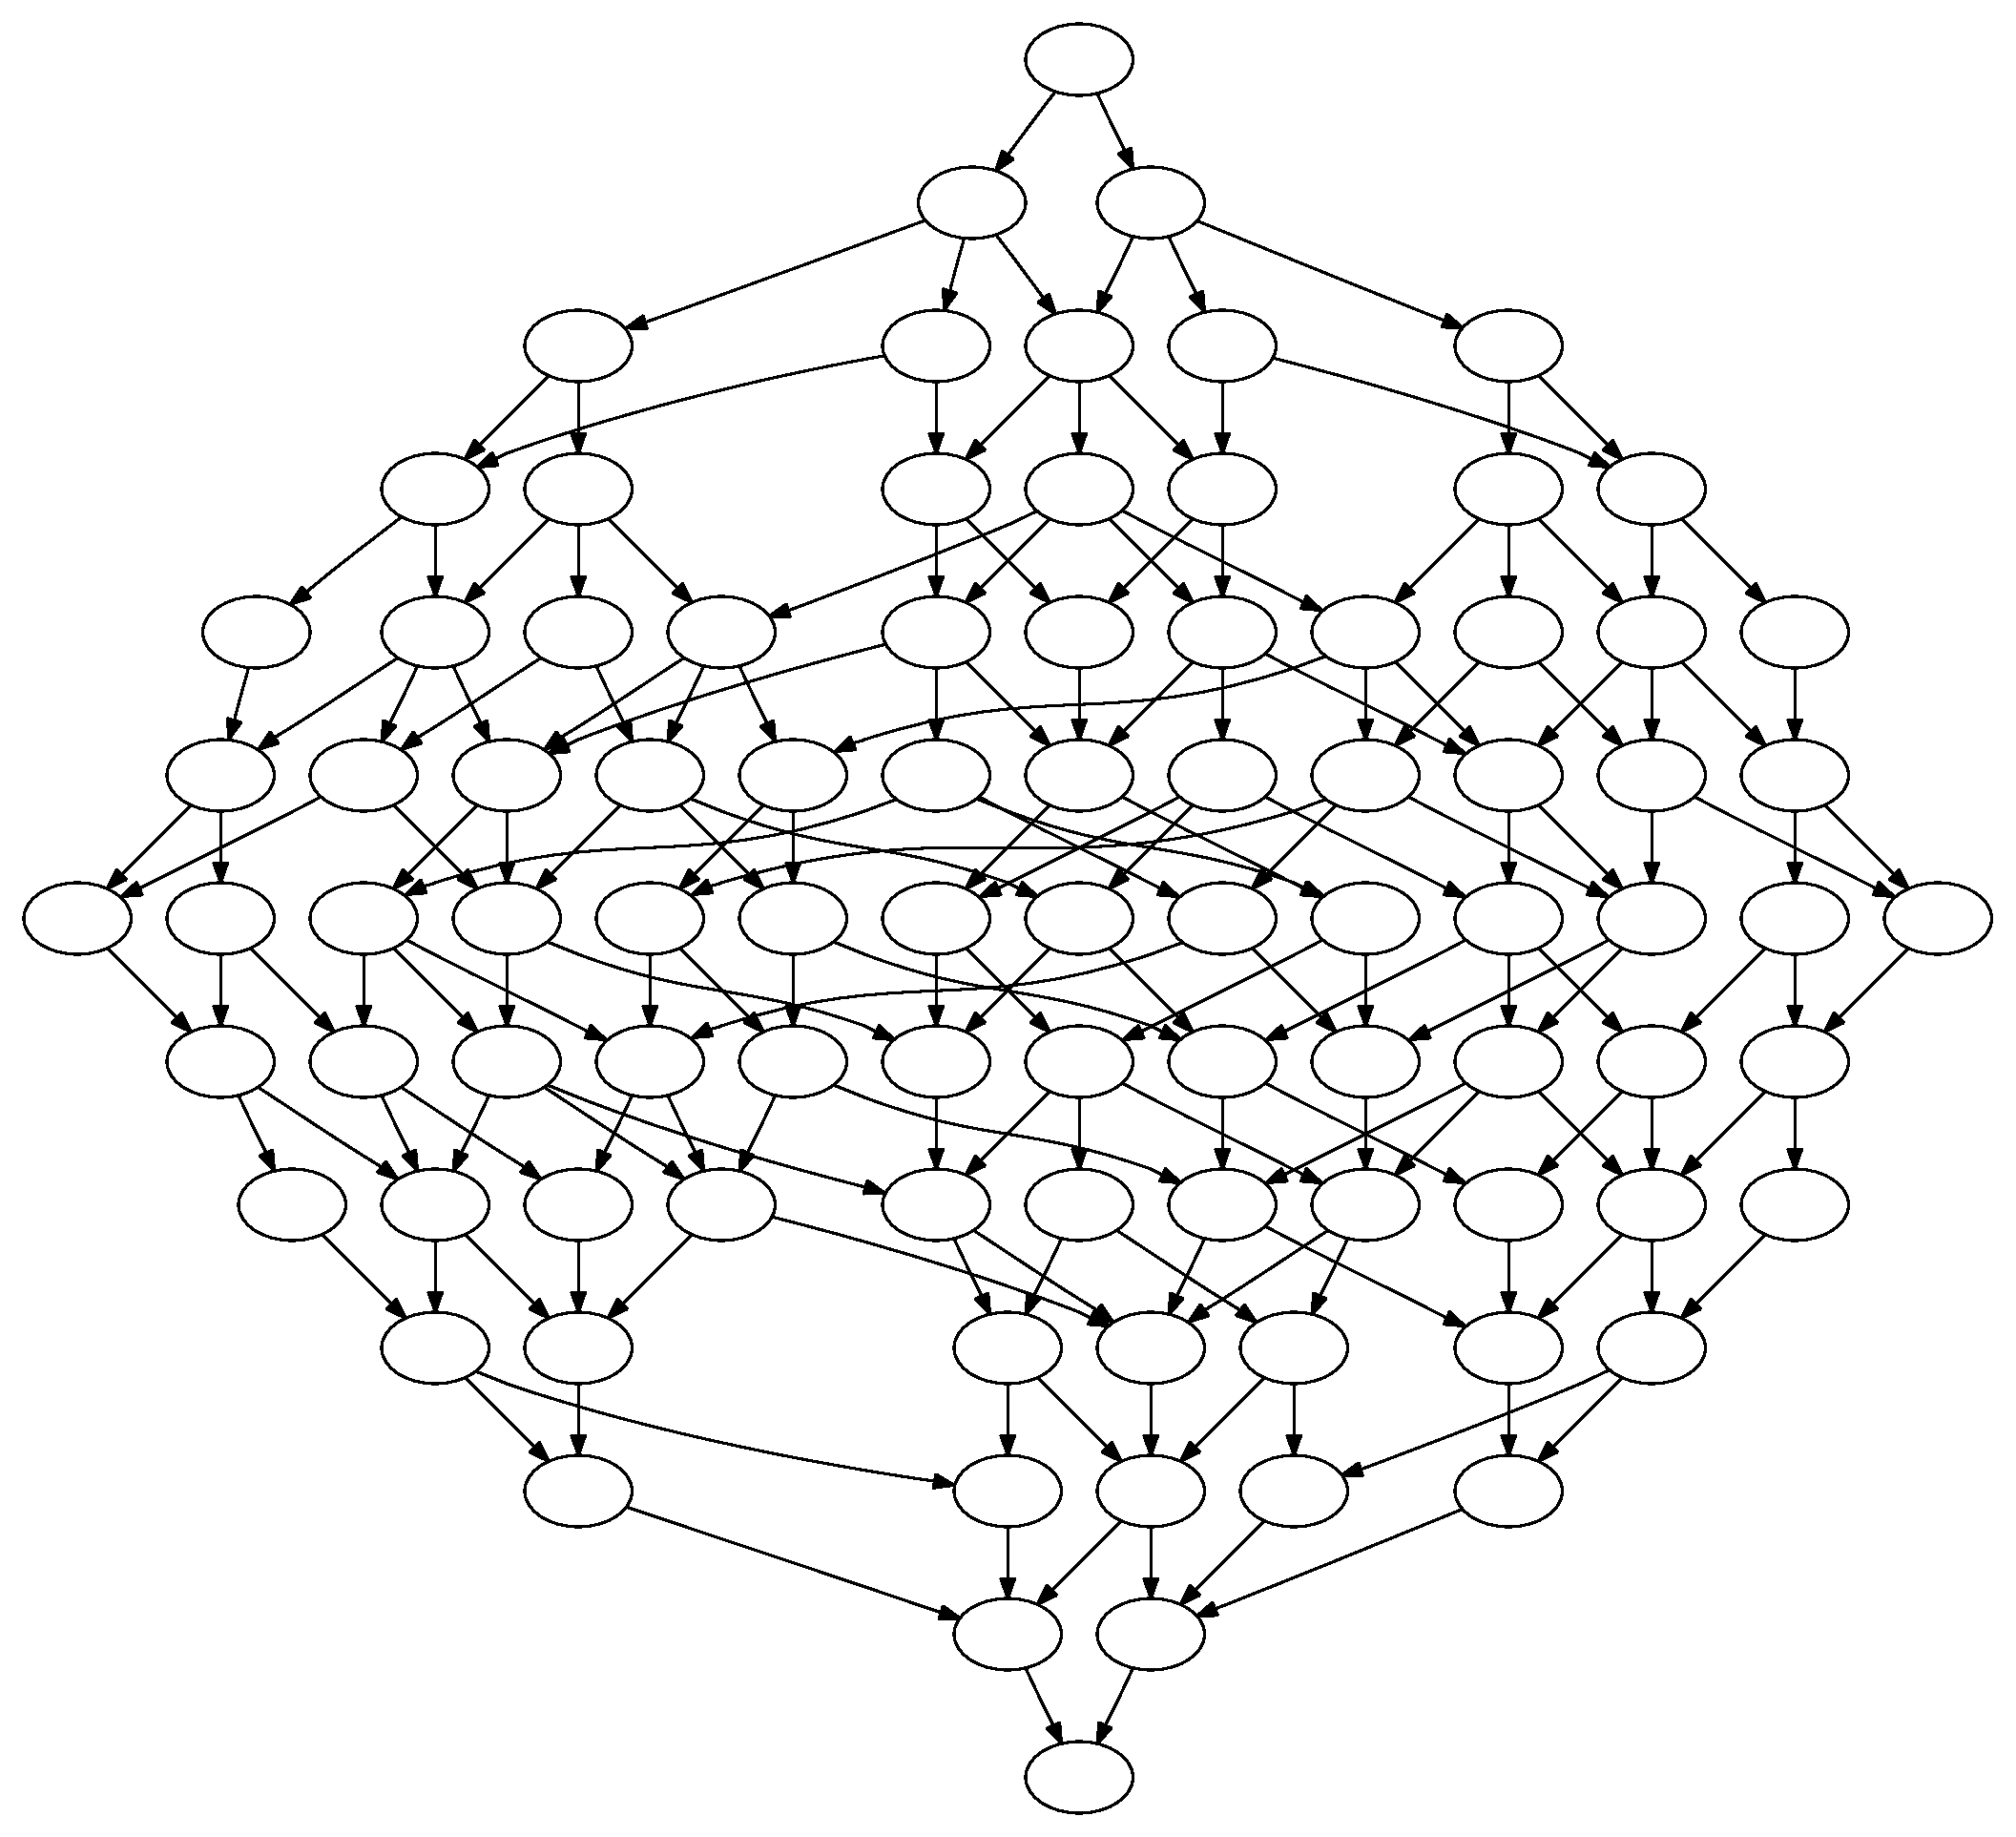
\includegraphics[width=0.30\textwidth]{sort-2,2,2.eps}}
    \caption{Graphs of increasing size.} \label{fig:sgrhs}
\end{figure}


The solution is constructed by propagating lists of integers along the edges of the graph with simple reduction rules at each vertex.  Ultimately, the elements of the list are combined in a weighted sum.

Graphs are characterized by a 3-tuple size, $(a,b,c)$, and list length, $d$.  The number of vertices, V, edges, E, layers, H, are:
$$ N = \left(a + b + c \atop a + b\right) \left(a + b \atop a\right) \qquad V = \frac{ab + ac + bc}{a + b + c} N \qquad H = ab + ac + bc $$
The average out-degree is given by $D = (ab + ac + bc) / (a+ b + c)$ and the maximum out degree by $M = a + b + c - \text{max}\{a,b,c\}$. The number of vertices in the largest layer, the width $W$, does not have a known analytic representation.  Graph sizes for the symmetric $a = b = c$ case are given in Table~\ref{tbl:size}. The amount of data attached to the graph is not known a-priori.  The $d$-length lists of integers on each edge contain arbitrary-precision integers, which can grow, requiring dynamic resizing. 
\begin{table}
\centering
\begin{tabular}{c | r r r r r}
S & V & E & W & H & M \\
\hline
1 & 6 & 6 & 2 & 3 & 2 \\
2 & 90 & 180 & 14 & 12 & 4 \\
3 & 1680 & 5040 & 142 & 27 & 6 \\
4 & 34650 & 138600 & 1968 & 48 & 8 \\
5 & 756756 & 3783780 & 31115 & 75 & 10 \\
6 & 17153136 & 102918816 & 542596 & 108 & 12 \\
7 & 399072960 & 2793510720 & 10083302 & 147 & 14 \\
8 & 9465511770 & 75724094160 & 196893250 & 192 & 16 \\
9 & 227873431500 & 2050860883500 & 3987935345 & 243 & 18
\end{tabular}
\caption{Number of vertices, $V$, number of edges, $E$, width, $W$, height, $H$, and maximal out-degree, $M$, for the first 9 symmetric, $a = b = c$, problems.}
\label{tbl:size}
\end{table}

\section*{Relevance}
Why should we think about counting tilings in a data intensive computing course? Many data intensive computing applications take the form of operations on a sparse graph.  These graphs are generally \textit{natural} in that they are derived from collections of natural processes, often human interaction.  If we consider the set of such natural graphs that can be downloaded and operated on, they sample the space of natural graphs very sparsely.  This can be seen by the examples given in Presto~\cite{Venkataraman2013}: only 5 data sets were operated on.

The graphs found in tiling problems share many characteristics with natural graphs: they have complex edge patterns and a distributions of degrees.  These graphs, however, don't come from collected data, but instead an \textit{analytic} expansion of a mathematical expression.  As such, they do a much better job of sampling the space of data sets.  In particular, the size, density, and width of a tiling problem can be controlled somewhat independently and varied more finely.  They can be scaled down small enough to be explicitly visualized, and large enough to fill any storage medium.  

The solution to large tiling problems is of additional interest. The current computational solution is a C with pthreads code that doesn't scale and has to be run on a shared memory supercomputer such as Blacklight at the PSC.  The time to solution for the $(8,8,8)$ problem is a couple of weeks, so coarse-grain check-pointing is needed to ensure resiliency.  Solutions based on an imperative paradigm with explicit virtual memory management and NUMA physical memory suffer from non-locality, with physical memory access patterns that look like random walks.  The $(9,9,9)$ problem is currently considered intractable.

I expect that implementations of tiling algorithms in a variety of data intensive computing frameworks would yield substantially better results at scale.  The algorithm is relatively simple, and could be implemented in Presto/Blokus, Graphlab/Graphchi, mapreduce, etc.  Tiling problems of different sizes and densities should reveal the strengths and weaknesses of the paradigms and back-end systems.  This knowledge would help inform future implementation decisions.  There is also the possibility that the wide variety of tests could reveal an unintended or otherwise correctable inefficiency in a data intensive computing system.



\begin{comment}


\end{comment}
\bibliographystyle{plain} 
\bibliography{../../../writings/bib/library}



\end{document}
